\documentclass[12pt]{article}
\usepackage{graphicx}
\usepackage{amsmath}
\usepackage{float}
\usepackage[backend=biber,sorting=none,style=apa]{biblatex}
\addbibresource{main.bib}

\usepackage{longtable}
\usepackage{pdfpages}
\usepackage{indentfirst}
\usepackage{setspace}
\onehalfspacing
\usepackage[margin=1in]{geometry}
\usepackage[hidelinks]{hyperref}
\usepackage{newtxtext}
\usepackage{newtxmath}

\usepackage{enumitem}
\usepackage{array}
\newlist{tableitemize}{itemize}{1}
\setlist[tableitemize]{
    label=\textbullet,
    leftmargin=*,
    topsep=0pt,
    partopsep=0pt,
    itemsep=0pt,
    parsep=0pt,
    before=\vspace{-6pt}
}

\newcolumntype{P}[1]{
    >{\raggedright\arraybackslash}p{#1}
}

\title{Title Here}
\author{Author Here}

\begin{document}

\pagenumbering{gobble}
\maketitle
\newpage

\pagenumbering{gobble}
\tableofcontents

\newpage

\pagenumbering{arabic}
% \input{} or content here.
\section{Part B}

\subsection{B-I Compare two approaches, two vendors}

In this section, customer refers to Company A.

\subsubsection{Resource Estimate}

Before comparing IaaS and PaaS, monthly resource requirements should be estimated at first. The requirements are shown in Table~\ref{tab:monthly-resource-requirement}.

\begin{table}[H]
	\centering
	\caption{Monthly Resource Requirement}
	\label{tab:monthly-resource-requirement}
	\begin{tabular}{|c|c|c|}
		\hline
		Resource                & Calculation                  & Monthly Requirement   \\
		\hline
		Survey submissions      & \(500 \times 30\)            & 15000 submissions     \\
		\hline
		Survey storage          & \(15000 \times 1 \text{KB}\) & 15 MB/month           \\
		\hline
		Peak requests per day   & \(50 \times 60 \times 10\)   & 30000 requests/day    \\
		\hline
		Peak requests per month & \(30000 \times 30\)          & 900000 requests/month \\
		\hline
		Daily reports           & \(1 \times 30\)              & 30 reports/month      \\
		\hline
	\end{tabular}
\end{table}

In addition, each submission must be retained for three years:
\begin{align*}
	500 \times 365 \times 3   & = 547500 \; \text{submissions} \\
	547500 \times 1 \text{KB} & = 547.5 \text{MB}
\end{align*}

Therefore, user data after three years is approximately 548 MB. The database capacity must also account for indexes, database storage overhead, and future growth. Assume that indexes require 20\% of the raw data size, database overhead requires 15\%, and a 25\% growth allowance is maintained, the estimated database size is:

\[
	548 \text{MB} \times 1.20 \times 1.15 \times 1.25 = 945.45 \text{MB}
\]

Therefore, the database is expected to require approximately 1 GB of storage. In this case, a minimum of 2 GB should be allocated for temporary operations, transaction logs, etc.

In addition to the production database, a backup policy is required to protect personal data against accidents. The proposed policy retains 30 daily backups for short-term recovery, and 36 monthly backups for the three-year retention period. An additional 36 monthly copies are stored in a separate region for disaster recovery. Assume that each backup contains approximately 1 GB, which is the estimated logical size of the database after three years. The backup storage requirement is:
\begin{align*}
	\text{Daily backups}       & = 30 \times 1 \text{GB} = 30 \text{GB} \\
	\text{Monthly backups}     & = 36 \times 1 \text{GB} = 36 \text{GB} \\
	\text{Cross-Region copies} & = 36 \times 1 \text{GB} = 36 \text{GB} \\
\end{align*}

Thus, the maximum backup storage requirement is:
\[
	30 \text{GB} + 36 \text{GB} + 36 \text{GB} = 102 \text{GB}
\]

Together with the 2 GB production database allocation, the conservative total storage requirement is:
\[
	2 \text{GB} + 102 \text{GB} = 104 \text{GB}
\]

\subsubsection{Comparison of IaaS and PaaS}

The comparison of IaaS and PaaS	is shown in Table~\ref{tab:comparison-iaas-paas}.

\begin{longtable}{|P{3.5cm}|P{6cm}|P{6cm}|}
	\caption{Comparison of IaaS and PaaS}
	\label{tab:comparison-iaas-paas}
	\endfirsthead
	\endhead

	\hline
	Criterion
	 & IaaS on vendor 1 \newline Amazon EC2
	 & PaaS on vendor 2 \newline Google Cloud Run
	\\
	\hline
	Who manages operating system (OS), runtime, scaling
	 &
	\begin{tableitemize}
		\item Operating System: Customer manages the guest OS.
		\item Runtime: Customer installs and manages it.
		\item Scaling: Customer defines and configures scaling, and AWS can execute it through EC2 Auto Scaling \parencite{aws_shared_responsibility_model, aws_ec2_scaling_methods}.
	\end{tableitemize}
	 &
	\begin{tableitemize}
		\item Operating System: Google manages the host OS, and the customer manages the container image.
		\item Runtime: Google manages the platform, which executes the container. The customer chooses the runtime included in the container.
		\item Scaling: Google manages scaling, and the customer configures its limits \parencite{google_cloud_run_container_contract, google_cloud_run_autoscaling}.
	\end{tableitemize}
	\\
	\hline
	Scaling behavior
	 &
	With EC2 Auto Scaling, it supports manual, scheduled, dynamic, and predictive scaling within configured minimum and maximum capacity. It can scale to zero if the minimum and desired capacity are set to zero \parencite{aws_ec2_scaling_methods, aws_ec2_auto_scaling_capacity_limits}
	 &
	It automatically scales container instances based on incoming requests, CPU utilization, and request concurrency. It scales to zero when idle, and starts new instances when requests arrive \parencite{google_cloud_run_autoscaling}.
	\\
	\hline
	Persistent storage or database option
	 &
	It supports persistent storage through Amazon EBS, EFS, FSx, or S3, as well as managed databases such as Amazon RDS \parencite{aws_ec2_storage_options, aws_amazon_rds}.
	 &
	It supports persistent storage through Cloud Storage volume mounts or NFS volume mounts, as well as managed databases such as Cloud SQL and Firestore \parencite{google_cloud_run_cloud_storage_volumes, google_cloud_run_nfs_mounts, google_cloud_run_cloud_sql, google_cloud_firestore}.
	\\
	\hline
	Identity and access control
	 &
	AWS Identity and Access Management (IAM) is an AWS service that helps an administrator securely control access to AWS resources. IAM administrators control who can be authenticated (signed in) and authorized (have permissions) to use Amazon EC2 resources \parencite{aws_ec2_identity_access_management}.
	 &
	By default, only project owners and editors can create, update, delete, or invoke Cloud Run resources, and only project owners and Cloud Run Admins can modify Identity and Access Management (IAM) policies \parencite{google_cloud_run_access_control}.
	\\
	\hline
	Logging and monitoring
	 &
	Use CloudWatch Logs to monitor applications and systems using log data from Amazon EC2 instances \parencite{aws_cloudwatch_logs}.
	 &
	Google Cloud Observability provides logging and monitoring tools that help you understand what is happening in your Cloud Run resource \parencite{google_cloud_run_monitoring}.
	\\
	\hline
	Regions available in or near Malaysia
	 &
	Asia Pacific (Malaysia) (\texttt{ap-southeast-5}), and Asia Pacific (Jakarta) (\texttt{ap-southeast-3}) \parencite{aws_regions}.
	 &
	Singapore (\texttt{asia-southeast1}), Indonesia (\texttt{asia-southeast2}), and Thailand (\texttt{asia-southeast3}) \parencite{google_region}.
	\\
	\hline
	Operating effort for a three-person IT team
	 &
	High effort for 3 IT staff, as the small IT team must manage EC2 instances, OS patching, scaling configuration, monitoring, backups, etc.
	 &
	Low effort for 3 IT staff, as Google Run is fully managed, so the small IT team could focus on maintaining and managing the survey platform itself, and ignore the underlying infrastructures.
	\\
	\hline
	Cost driver
	 &
	Instance type, region, EBS storage \parencite{aws_calculator}.
	 &
	Request count, selected region, Cloud SQL, Cloud Storage \parencite{google_cloud_pricing_calculator}.
	\\
	\hline
\end{longtable}

\subsubsection{Monthly Cost Estimate}

The monthly cost estimate of IaaS solution using Amazon EC2 is totally 21.49 USD, and the detail configuration is shown in Table~\ref{tab:monthly-estimate-of-amazon-ec2}.

\begin{table}[H]
	\centering
	\caption{Monthly Estimate of Amazon EC2 (Accessed 2026-11-12)}
	\label{tab:monthly-estimate-of-amazon-ec2}
	\begin{tabular}{|P{5cm}|P{2cm}|P{5cm}|P{2cm}|}
		\hline
		Service
		 & Region
		 & Type/Size
		 & Monthly Cost (USD)
		\\
		\hline
		Amazon EC2
		 & Malaysia
		 & t3.small with 20 GB EBS
		 & 19.10
		\\
		\hline
		Amazon Simple Storage Service (S3) for primary backup
		 & Malaysia
		 & 66 GB
		 & 1.49
		\\
		\hline
		Amazon Simple Storage Service (S3) for cross-region backup
		 & Singapore
		 & 36 GB
		 & 0.90
		\\
		\hline
	\end{tabular}
\end{table}

The monthly cost estimate of PaaS solution using Google Cloud Run is overall 27.44 USD, and the detail configuration is shown in Table~\ref{tab:monthly-estimate-of-google-cloud-run}.

\begin{table}[H]
	\centering
	\caption{Monthly Estimate of Google Cloud Run (Accessed 2026-11-12)}
	\label{tab:monthly-estimate-of-google-cloud-run}
	\begin{tabular}{|P{4cm}|P{2cm}|P{5cm}|P{2cm}|}
		\hline
		Service
		 & Region
		 & Type/Size
		 & Monthly Cost (USD)
		\\
		\hline
		Cloud Run
		 & Singapore
		 & Stead traffic shape and 1 million requests per month
		 & 14.14
		\\
		\hline
		Cloud SQL
		 & Singapore
		 & PostgreSQL, db-f1-micro, 10 GB
		 & 13.11
		\\
		\hline
		Cloud Storage for primary backup
		 & Singapore
		 & Archive Storage, 66 GB
		 & 0.10
		\\
		\hline
		Cloud Storage for cross-region backup
		 & Jakarta
		 & Archive Storage, 36 GB
		 & 0.09
		\\
		\hline
	\end{tabular}
\end{table}

\subsubsection{Recommendation}

Overall, the PaaS solution is recommended. Although its estimated monthly cost is higher than that of the IaaS solution, the additional cost is justified as it reduces responsibilities for managing infrastructures. The PaaS provider manages the underlying infrastructure, operating system, and automatic scaling, which allows the three-person IT team to focus on the survey platform, access control, data protection, monitoring, etc. In contrast, the IaaS solution would require the same team to manage both the infrastructure and the survey platform. Therefore, PaaS provides a more sustainable and operationally suitable solution for company A.

\subsection{B-II Design and justify}

\subsubsection{Architecture Diagram}

The proposed architecture of the cloud survey platform is shown in Figure~\ref{fig:cloud-architecture}.

\begin{figure}[H]
	\centering
	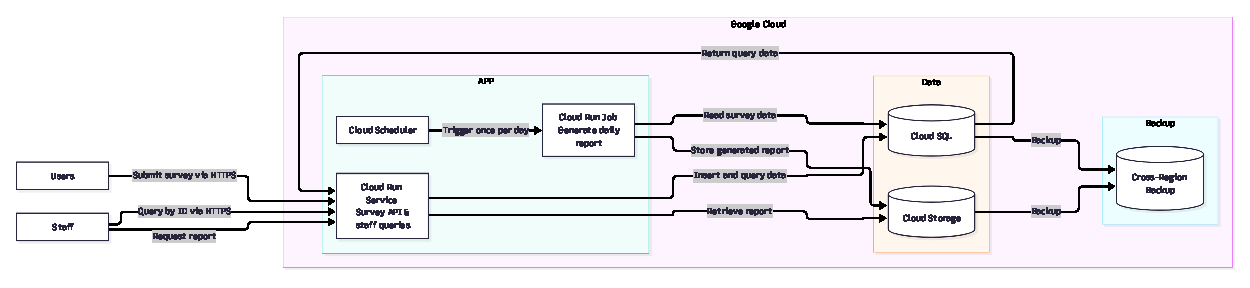
\includegraphics[width=\textwidth]{img/architecture.pdf}
	\caption{Architecture of the Cloud Survey Platform}
	\label{fig:cloud-architecture}
\end{figure}


\thispagestyle{empty}
\phantomsection
\setcounter{page}{1}
\renewcommand{\thepage}{A\arabic{page}}
\addcontentsline{toc}{section}{List of References}
\printbibliography
\newpage

\end{document}
